\documentclass[12pt,a4paper]{article}

% ── Packages ──
\usepackage[utf8]{inputenc}
\usepackage[T1]{fontenc}
\usepackage{amsmath,amssymb}
\usepackage{geometry}
\usepackage{graphicx}
\usepackage{booktabs}
\usepackage{array}
\usepackage{enumitem}
\usepackage{hyperref}
\usepackage{xcolor}
\usepackage{listings}
\usepackage{fancyhdr}
\usepackage{titlesec}
\usepackage{tcolorbox}
\usepackage{tikz}
\usepackage{pgfplots}
\pgfplotsset{compat=1.18}

\geometry{margin=2.5cm}
\hypersetup{colorlinks=true, linkcolor=blue!60!black, urlcolor=blue!60!black}

% ── Header / Footer ──
\pagestyle{fancy}
\fancyhf{}
\fancyhead[L]{\textit{Filters, Transfer Functions \& Anti-Aliasing}}
\fancyhead[R]{\textit{GNC Fundamentals}}
\fancyfoot[C]{\thepage}

% ── Custom box ──
\newtcolorbox{keybox}[1][]{colback=blue!5!white, colframe=blue!50!black,
  fonttitle=\bfseries, title=#1}

\newtcolorbox{warningbox}[1][]{colback=red!5!white, colframe=red!50!black,
  fonttitle=\bfseries, title=#1}

% ── Title ──
\title{\textbf{Filters, Transfer Functions \& Anti-Aliasing}\\[0.5em]
       \large A Comprehensive Guide for GNC Engineers}
\author{}
\date{March 2026}

\begin{document}
\maketitle
\tableofcontents
\newpage

% ══════════════════════════════════════════════════════════════════════════════
\section{What is a Filter?}
% ══════════════════════════════════════════════════════════════════════════════

A filter is a system that \textbf{selectively allows certain frequencies} of a signal to pass through while \textbf{attenuating (reducing) others}. Think of it like a sieve---but for frequencies instead of particle sizes.

% ══════════════════════════════════════════════════════════════════════════════
\section{Low-Pass Filter (LPF)}
% ══════════════════════════════════════════════════════════════════════════════

A low-pass filter \textbf{passes low frequencies and blocks high frequencies}.

\begin{itemize}
    \item \textbf{Below the cutoff frequency} $f_c$: signal passes through (mostly unchanged).
    \item \textbf{Above the cutoff frequency} $f_c$: signal is attenuated (weakened).
\end{itemize}

\textbf{Use cases:} Smoothing noisy sensor data, removing high-frequency vibration from a control signal, anti-aliasing before sampling.

\textbf{Analogy:} A heavy blanket on a drum---slow (low-frequency) movements pass, but fast vibrations are absorbed.

% ══════════════════════════════════════════════════════════════════════════════
\section{High-Pass Filter (HPF)}
% ══════════════════════════════════════════════════════════════════════════════

A high-pass filter \textbf{passes high frequencies and blocks low frequencies}. The opposite of a low-pass filter.

\begin{itemize}
    \item \textbf{Above} $f_c$: signal passes.
    \item \textbf{Below} $f_c$: signal is attenuated.
\end{itemize}

\textbf{Use cases:} Removing DC offset or slow drift from a signal, extracting fast-changing dynamics.

\textbf{Analogy:} A stiff spring---it responds to fast jerky inputs but ignores slow steady pushes.

% ══════════════════════════════════════════════════════════════════════════════
\section{Fundamentals of the Cutoff Frequency}
% ══════════════════════════════════════════════════════════════════════════════

\subsection{Definition}

The cutoff frequency $f_c$ (also called \textbf{corner frequency}, \textbf{break frequency}, or \textbf{$-3$\,dB frequency}) is the frequency at which a filter's output power drops to \textbf{half} of its passband (maximum) power. Equivalently, the output amplitude drops to $\frac{1}{\sqrt{2}} \approx 0.707$ of the passband amplitude:

\begin{equation}
    |H(j\omega_c)| = \frac{1}{\sqrt{2}} \quad \Longleftrightarrow \quad -3\;\text{dB}
\end{equation}

\subsection{What It Physically Represents}

The cutoff frequency is the \textbf{boundary between two regions}:

\begin{center}
\begin{tabular}{lll}
    \toprule
    \textbf{Region} & \textbf{Frequency Range} & \textbf{What Happens} \\
    \midrule
    Passband  & $f < f_c$ (for low-pass) & Signal passes with little or no attenuation \\
    Stopband  & $f > f_c$ (for low-pass) & Signal is progressively attenuated \\
    \bottomrule
\end{tabular}
\end{center}

$f_c$ is not a hard wall---it is a \textbf{transition point}. The filter does not suddenly switch from ``pass'' to ``block'' at $f_c$. Instead, attenuation increases gradually, and $f_c$ marks where it becomes significant.

\subsection{Two Equivalent Ways to Express It}

\begin{enumerate}
    \item \textbf{In frequency (Hz):} $f_c \;[\text{Hz}]$
    \item \textbf{In angular frequency (rad/s):} $\omega_c = 2\pi f_c \;[\text{rad/s}]$
\end{enumerate}

Transfer functions typically use $\omega_c$ because the math is cleaner. Datasheets and practical specifications typically use $f_c$.

\subsection{How It Relates to the Transfer Function}

For a first-order low-pass filter:
\begin{equation}
    H(s) = \frac{\omega_c}{s + \omega_c} = \frac{1}{\tau s + 1}
\end{equation}

The cutoff frequency is directly encoded in the denominator. The pole is at $s = -\omega_c$, and:
\begin{equation}
    \tau = \frac{1}{\omega_c} = \frac{1}{2\pi f_c}
\end{equation}
where $\tau$ is the \textbf{time constant}---the time-domain equivalent of $f_c$.

\subsection{Relationship Between $f_c$ and Time Constant $\tau$}

These are two sides of the same coin:
\begin{equation}
    f_c = \frac{1}{2\pi\tau} \qquad \Longleftrightarrow \qquad \tau = \frac{1}{2\pi f_c}
\end{equation}

\begin{center}
\begin{tabular}{lll}
    \toprule
    \textbf{Parameter} & \textbf{Domain} & \textbf{Meaning} \\
    \midrule
    $f_c$ & Frequency domain & Frequency where attenuation starts \\
    $\tau$ & Time domain & Time for step response to reach 63\% \\
    \bottomrule
\end{tabular}
\end{center}

\begin{itemize}
    \item \textbf{Higher $f_c$} = smaller $\tau$ = faster response, lets more frequencies through.
    \item \textbf{Lower $f_c$} = larger $\tau$ = slower response, heavier smoothing.
\end{itemize}

\subsection{Behaviour at Three Key Frequencies}

For a single-pole low-pass filter:

\begin{center}
\begin{tabular}{lcccc}
    \toprule
    \textbf{Frequency} & \textbf{Gain $|H|$} & \textbf{Gain (dB)} & \textbf{Phase Shift} & \textbf{Physical Meaning} \\
    \midrule
    $f \ll f_c$  & $\approx 1$                    & $\approx 0$\,dB     & $\approx 0°$  & Signal passes unchanged \\
    $f = f_c$    & $\frac{1}{\sqrt{2}}$           & $-3$\,dB            & $-45°$        & Half-power point (cutoff) \\
    $f \gg f_c$  & $\approx \frac{f_c}{f} \to 0$  & $\to -\infty$       & $\to -90°$    & Signal strongly attenuated \\
    \bottomrule
\end{tabular}
\end{center}

\subsection{How to Choose the Cutoff Frequency}

The choice of $f_c$ depends on the application.

\textbf{Rule of thumb:} Set $f_c$ above the highest frequency you care about, but below the frequencies you want to reject:
\begin{equation}
    f_{\text{signal,\,max}} \;<\; f_c \;<\; f_{\text{noise,\,min}}
\end{equation}

\textbf{Example:} Useful signal occupies 0--20\,Hz, noise starts around 60\,Hz. Set $f_c \approx 30\text{--}40$\,Hz. This preserves the signal while attenuating the noise.

\begin{center}
\begin{tabular}{ll}
    \toprule
    \textbf{If $f_c$ is too high\ldots} & \textbf{If $f_c$ is too low\ldots} \\
    \midrule
    Noise passes through             & Useful signal gets attenuated \\
    Poor filtering                   & Slow response, phase lag \\
    Signal is clean but noisy        & Signal is smooth but distorted/delayed \\
    \bottomrule
\end{tabular}
\end{center}

\subsection{Cutoff Frequency in Hardware (RC Circuit)}

For a simple RC low-pass filter (resistor + capacitor):
\begin{equation}
    f_c = \frac{1}{2\pi RC}
\end{equation}

\begin{itemize}
    \item Want \textbf{lower} $f_c$? Increase $R$ or $C$ $\to$ more smoothing, slower response.
    \item Want \textbf{higher} $f_c$? Decrease $R$ or $C$ $\to$ less smoothing, faster response.
\end{itemize}

\subsection{Cutoff Frequency in Digital Filters}

In a digital (discrete-time) system running at sample rate $f_s$, the cutoff frequency must satisfy:
\begin{equation}
    f_c < \frac{f_s}{2}
\end{equation}

A common discrete approximation of a first-order low-pass filter is the \textbf{exponential moving average}:
\begin{equation}
    y[n] = \alpha \cdot x[n] + (1 - \alpha) \cdot y[n-1]
\end{equation}

where the smoothing factor $\alpha$ relates to $f_c$ by:
\begin{equation}
    \alpha = \frac{2\pi f_c \,\Delta t}{1 + 2\pi f_c\, \Delta t}
           = \frac{2\pi f_c / f_s}{1 + 2\pi f_c / f_s}
\end{equation}

\begin{itemize}
    \item $\alpha \to 1$: no filtering (output $=$ input).
    \item $\alpha \to 0$: heavy filtering (output barely changes).
\end{itemize}

\subsection{Cutoff Frequency on a Bode Plot}

On a Bode magnitude plot, $f_c$ is located where the two straight-line asymptotes---the flat passband and the $-20$\,dB/decade slope---\textbf{intersect}. This is why $f_c$ is also called the ``corner frequency.''

\begin{figure}[ht]
\centering
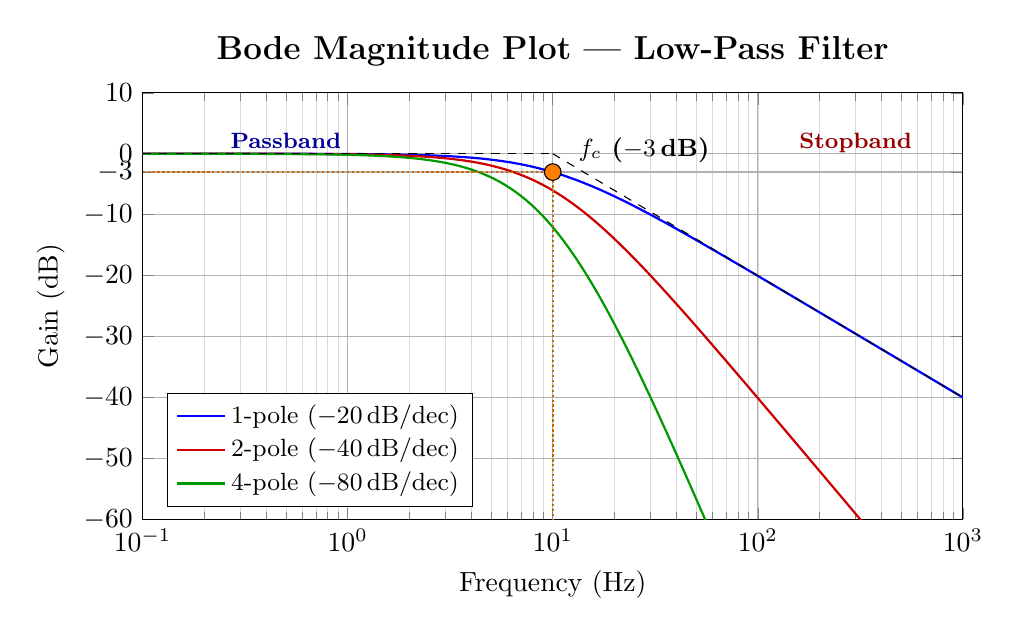
\begin{tikzpicture}
\begin{semilogxaxis}[
    width=12cm, height=7cm,
    xlabel={Frequency (Hz)},
    ylabel={Gain (dB)},
    xmin=0.1, xmax=1000,
    ymin=-60, ymax=10,
    grid=both,
    grid style={line width=0.2pt, draw=gray!30},
    major grid style={line width=0.4pt, draw=gray!60},
    ytick={10, 0, -3, -10, -20, -30, -40, -50, -60},
    legend pos=south west,
    legend style={font=\small},
    title={\textbf{Bode Magnitude Plot --- Low-Pass Filter}},
    title style={font=\large},
]

% ── Actual 1st-order response: 20*log10(1/sqrt(1+(f/fc)^2)), fc=10 ──
\addplot[
    blue, thick, smooth, domain=0.1:1000, samples=200
] {20*log10(1/sqrt(1+(x/10)^2))};
\addlegendentry{1-pole ($-20$\,dB/dec)}

% ── Actual 2nd-order response: 20*log10(1/(1+(f/fc)^2)), fc=10 ──
\addplot[
    red!80!black, thick, smooth, domain=0.1:1000, samples=200
] {20*log10(1/(1+(x/10)^2))};
\addlegendentry{2-pole ($-40$\,dB/dec)}

% ── Actual 4th-order response ──
\addplot[
    green!60!black, thick, smooth, domain=0.1:1000, samples=200
] {20*log10(1/( (1+(x/10)^2)^2 ))};
\addlegendentry{4-pole ($-80$\,dB/dec)}

% ── Asymptotes (dashed) ──
\addplot[
    black, dashed, thin, domain=0.1:10
] {0};
\addplot[
    black, dashed, thin, domain=10:1000
] {-20*log10(x/10)};

% ── Cutoff frequency marker ──
\addplot[
    only marks, mark=*, mark size=3pt, black, fill=orange
] coordinates {(10, -3.01)};

% ── Annotations ──
\node[anchor=south west, font=\small\bfseries] at (axis cs:12, -3.01)
    {$f_c$ ($-3$\,dB)};

\draw[densely dotted, thick, orange!80!black]
    (axis cs:0.1, -3.01) -- (axis cs:10, -3.01) -- (axis cs:10, -60);

\node[anchor=north, font=\footnotesize, text=blue!60!black] at (axis cs:0.5, 5)
    {\textbf{Passband}};
\node[anchor=north, font=\footnotesize, text=red!60!black] at (axis cs:300, 5)
    {\textbf{Stopband}};

\end{semilogxaxis}
\end{tikzpicture}
\caption{Bode magnitude plot of low-pass filters with $f_c = 10$\,Hz. The orange dot marks the $-3$\,dB cutoff point. Higher-order (multi-pole) filters have steeper roll-off in the stopband.}
\label{fig:bode_cutoff}
\end{figure}

\begin{keybox}[Cutoff Frequency Summary]
\centering
\begin{tabular}{ll}
    \toprule
    \textbf{Concept} & \textbf{Key Fact} \\
    \midrule
    What            & Frequency where output power $=$ half of input power \\
    Value           & $|H| = 1/\sqrt{2} \approx 0.707$ ($-3$\,dB) \\
    Time-domain eq. & $\tau = 1/(2\pi f_c)$ \\
    In the TF       & Equals the pole location: $\omega_c$ \\
    On a Bode plot  & The corner where the two asymptotes meet \\
    Design rule     & Set above signal bandwidth, below noise frequencies \\
    \bottomrule
\end{tabular}
\end{keybox}

% ══════════════════════════════════════════════════════════════════════════════
\section{Why $-3$\,dB?}
% ══════════════════════════════════════════════════════════════════════════════

The $-3$\,dB point comes from a specific physical meaning: it is where the output \textbf{power} is exactly \textbf{half} of the input power.

\subsection{The Power Definition}

Decibels for power are defined as:
\begin{equation}
    \text{dB} = 10\,\log_{10}\!\left(\frac{P_{\text{out}}}{P_{\text{in}}}\right)
\end{equation}

At half power:
\begin{equation}
    10\,\log_{10}\!\left(\frac{1}{2}\right) = 10 \times (-0.3010) = -3.010\;\text{dB}
\end{equation}

\subsection{Amplitude Interpretation}

Since power is proportional to amplitude squared ($P \propto V^2$), half power corresponds to an amplitude ratio of:
\begin{equation}
    \frac{V_{\text{out}}}{V_{\text{in}}} = \sqrt{\frac{1}{2}} = \frac{1}{\sqrt{2}} \approx 0.707
\end{equation}

Verification using the amplitude dB formula:
\begin{equation}
    20\,\log_{10}\!\left(\frac{1}{\sqrt{2}}\right) = 20 \times (-0.1505) = -3.01\;\text{dB}
\end{equation}

\subsection{Why Half-Power is the Natural Breakpoint}

For a single-pole low-pass filter:
\begin{equation}
    H(s) = \frac{\omega_c}{s + \omega_c}
\end{equation}

Evaluate the magnitude at $\omega = \omega_c$:
\begin{equation}
    |H(j\omega_c)| = \frac{\omega_c}{\sqrt{\omega_c^2 + \omega_c^2}}
                    = \frac{\omega_c}{\omega_c\sqrt{2}}
                    = \frac{1}{\sqrt{2}}
\end{equation}

At the frequency where $\omega$ \textbf{equals} the pole location $\omega_c$, the gain is always $\frac{1}{\sqrt{2}}$. This is the natural ``corner'' of the filter---where the two asymptotes of the Bode plot intersect. Half-power ($-3$\,dB) is not an arbitrary convention; it is the \textbf{inherent mathematical breakpoint} of the filter's transfer function.

\begin{keybox}[Summary Table]
\centering
\begin{tabular}{ll}
    \toprule
    \textbf{Fact} & \textbf{Value} \\
    \midrule
    $-3$\,dB in power & $P_{\text{out}}/P_{\text{in}} = 1/2$ (half power) \\
    $-3$\,dB in amplitude & $V_{\text{out}}/V_{\text{in}} = 1/\sqrt{2} \approx 0.707$ \\
    Why this value? & $\omega = \omega_c$ in the transfer function---the natural corner \\
    \bottomrule
\end{tabular}
\end{keybox}

% ══════════════════════════════════════════════════════════════════════════════
\section{Transfer Function and Its Relation to Filters}
% ══════════════════════════════════════════════════════════════════════════════

\subsection{What is a Transfer Function?}

A transfer function $H(s)$ is a \textbf{mathematical representation} of a system's input--output relationship in the \textbf{Laplace domain} (s-domain):

\begin{equation}
    H(s) = \frac{Y(s)}{X(s)}
\end{equation}

where:
\begin{itemize}
    \item $Y(s)$ = output (Laplace transform),
    \item $X(s)$ = input (Laplace transform),
    \item $s = \sigma + j\omega$ is the complex frequency variable.
\end{itemize}

\subsection{How It Relates to Filters}

\textbf{Every filter IS a transfer function.} The transfer function defines \emph{how} each frequency is treated:

\begin{center}
\begin{tabular}{lll}
    \toprule
    \textbf{Filter Type} & \textbf{Transfer Function} & \textbf{Behavior} \\
    \midrule
    Low-Pass  & $\displaystyle H(s) = \frac{\omega_c}{s + \omega_c}$ & Gain $\to 1$ at low freq, $\to 0$ at high freq \\[1em]
    High-Pass & $\displaystyle H(s) = \frac{s}{s + \omega_c}$        & Gain $\to 0$ at low freq, $\to 1$ at high freq \\
    \bottomrule
\end{tabular}
\end{center}

where $\omega_c = 2\pi f_c$ is the cutoff frequency in rad/s.

\subsection{Frequency Response}

To see how a filter behaves at a specific frequency, substitute $s = j\omega$.

\textbf{Low-Pass example:}
\begin{equation}
    H(j\omega) = \frac{\omega_c}{j\omega + \omega_c}
\end{equation}

The magnitude is:
\begin{equation}
    |H(j\omega)| = \frac{\omega_c}{\sqrt{\omega^2 + \omega_c^2}}
\end{equation}

\begin{itemize}
    \item When $\omega \ll \omega_c$: $|H| \approx 1$ \quad (signal passes)
    \item When $\omega = \omega_c$: $|H| = \frac{1}{\sqrt{2}}$ \quad ($-3$\,dB point)
    \item When $\omega \gg \omega_c$: $|H| \approx \frac{\omega_c}{\omega} \to 0$ \quad (signal blocked)
\end{itemize}

% ══════════════════════════════════════════════════════════════════════════════
\section{Single-Pole vs.\ Multi-Pole Low-Pass Filters}
% ══════════════════════════════════════════════════════════════════════════════

\subsection{What is a ``Pole''?}

A \textbf{pole} is a root of the \textbf{denominator} of the transfer function. It determines how aggressively the filter rolls off (attenuates) at high frequencies.

In $H(s) = \dfrac{\omega_c}{s + \omega_c}$, the denominator $s + \omega_c = 0$ gives the pole at $s = -\omega_c$.

\subsection{Single-Pole (First-Order) Low-Pass Filter}

\textbf{Transfer function:}
\begin{equation}
    H(s) = \frac{\omega_c}{s + \omega_c}
         = \frac{1}{\dfrac{s}{\omega_c} + 1}
         = \frac{1}{\tau s + 1}
\end{equation}

where $\tau = \dfrac{1}{\omega_c}$ is the \textbf{time constant}.

\begin{keybox}[Key Characteristics]
\centering
\begin{tabular}{ll}
    \toprule
    \textbf{Property} & \textbf{Value} \\
    \midrule
    Roll-off rate           & $-20$\,dB/decade ($-6$\,dB/octave) \\
    Phase shift at $f_c$    & $-45°$ \\
    Maximum phase shift     & $-90°$ \\
    Number of poles         & 1 \\
    \bottomrule
\end{tabular}
\end{keybox}

\textbf{Roll-off meaning:} Above the cutoff, every time the frequency increases by $10\times$, the output drops by 20\,dB (a factor of 10 in amplitude).

\textbf{Time domain:} The step response is an exponential rise:
\begin{equation}
    y(t) = 1 - e^{-t/\tau}
\end{equation}
It reaches $\sim$63\% of the final value after one time constant $\tau$.

\textbf{Pros:} Simple, no overshoot, always stable. \\
\textbf{Cons:} Gentle roll-off---doesn't reject high frequencies very sharply.

\subsection{Multi-Pole (Higher-Order) Low-Pass Filters}

Adding more poles makes the filter \textbf{steeper} (sharper cutoff).

\subsubsection{Second-Order (2-Pole) Low-Pass Filter}

\begin{equation}
    H(s) = \frac{\omega_n^2}{s^2 + 2\zeta\omega_n s + \omega_n^2}
\end{equation}

where:
\begin{itemize}
    \item $\omega_n$ = natural frequency,
    \item $\zeta$ = damping ratio (controls overshoot/ringing).
\end{itemize}

\textbf{Roll-off:} $-40$\,dB/decade (twice as steep).

\subsubsection{$N$-th Order ($N$-Pole) Low-Pass Filter}

General form:
\begin{equation}
    H(s) = \frac{\omega_c^N}{\displaystyle\prod_{i=1}^{N}(s + p_i)}
    \qquad\text{or}\qquad
    H(s) = \frac{1}{(\tau s + 1)^N} \;\text{(Butterworth-like)}
\end{equation}

\begin{center}
\begin{tabular}{ccc}
    \toprule
    \textbf{Order (Poles)} & \textbf{Roll-off Rate} & \textbf{Phase at $f_c$} \\
    \midrule
    1 & $-20$\,dB/decade  & $-45°$  \\
    2 & $-40$\,dB/decade  & $-90°$  \\
    3 & $-60$\,dB/decade  & $-135°$ \\
    $N$ & $-20N$\,dB/decade & $-N \times 45°$ \\
    \bottomrule
\end{tabular}
\end{center}

\subsection{Trade-offs of More Poles}

\begin{center}
\begin{tabular}{lll}
    \toprule
    & \textbf{Single-Pole} & \textbf{Multi-Pole} \\
    \midrule
    Roll-off    & Gentle ($-20$\,dB/dec)  & Sharp ($-20N$\,dB/dec) \\
    Phase lag   & Less (max $-90°$)       & More (max $-N\times 90°$) \\
    Stability   & Always stable           & Can oscillate if poorly tuned \\
    Overshoot   & None                    & Possible (depends on $\zeta$) \\
    Delay       & Less                    & More group delay \\
    Complexity  & Simple                  & More computation/components \\
    \bottomrule
\end{tabular}
\end{center}

% ══════════════════════════════════════════════════════════════════════════════
\section{What Does ``A Signal Contains Frequencies'' Mean?}
% ══════════════════════════════════════════════════════════════════════════════

\subsection{Fourier's Theorem}

Any real-world signal---no matter how complex---can be decomposed into a \textbf{sum of sine waves} at different frequencies. This is Fourier's theorem.

For example, a vibration sensor output might be:
\begin{equation}
    x(t) = \underbrace{3\sin(2\pi \cdot 10\, t)}_{\text{10\,Hz component}}
          + \underbrace{1.5\sin(2\pi \cdot 50\, t)}_{\text{50\,Hz component}}
          + \underbrace{0.2\sin(2\pi \cdot 300\, t)}_{\text{300\,Hz component}}
          + \cdots
\end{equation}

This signal ``contains'' frequencies of 10\,Hz, 50\,Hz, 300\,Hz, etc. Each is a building block of the total signal.

% ══════════════════════════════════════════════════════════════════════════════
\section{Digitizing a Signal}
% ══════════════════════════════════════════════════════════════════════════════

\subsection{The Real World is Continuous}

A physical signal---like the voltage from a sensor---exists \textbf{continuously} in time. At every instant it has a value. This is an \textbf{analog signal}: smooth, unbroken, and existing in nature.

\subsection{Computers Need Discrete Numbers}

A computer cannot store infinitely many values. To get a real-world signal into a computer, you must convert it from analog to digital. This is \textbf{digitizing}.

\subsection{How Digitizing Works}

A device called an \textbf{ADC (Analog-to-Digital Converter)} performs two steps:

\begin{enumerate}
    \item \textbf{Sampling} --- Measure the signal's value at regular intervals, spaced $T_s = 1/f_s$ seconds apart. If $f_s = 1000$\,Hz, you take 1000 measurements per second, one every 1\,ms.

    \item \textbf{Quantization} --- Round each measurement to a finite precision. The continuous voltage (e.g., 2.3471928\ldots\,V) gets rounded to the nearest representable value (e.g., 2.347\,V with a 12-bit ADC).
\end{enumerate}

\begin{keybox}[Key Terms]
\centering
\begin{tabular}{ll}
    \toprule
    \textbf{Term} & \textbf{Meaning} \\
    \midrule
    Analog signal & Continuous---exists at every instant in time \\
    Digitize & Convert into a sequence of numbers a computer can store \\
    Sampling & Measuring the signal at fixed time intervals \\
    Sample rate $f_s$ & How many measurements per second \\
    ADC & The hardware that performs this conversion \\
    \bottomrule
\end{tabular}
\end{keybox}

% ══════════════════════════════════════════════════════════════════════════════
\section{Anti-Aliasing}
% ══════════════════════════════════════════════════════════════════════════════

\subsection{The Problem: Aliasing}

When you \textbf{sample} a continuous signal at discrete time intervals, you are only capturing snapshots. If the signal contains frequencies \textbf{higher than half your sampling rate}, those high frequencies get misidentified as \textbf{lower frequencies} in the sampled data.

This is \textbf{aliasing}---a high-frequency signal masquerading as a low-frequency one. Once it happens, it \textbf{cannot be undone}.

\subsection{The Nyquist--Shannon Theorem}

To correctly capture a frequency $f$, you must sample at a rate:
\begin{equation}
    f_s > 2f
\end{equation}

The critical boundary $f_s/2$ is called the \textbf{Nyquist frequency} $f_N$:
\begin{equation}
    f_N = \frac{f_s}{2}
\end{equation}

\begin{itemize}
    \item Frequencies \textbf{below} $f_N$: correctly captured.
    \item Frequencies \textbf{above} $f_N$: aliased (folded back into the $0$ to $f_N$ range).
\end{itemize}

\subsection{Aliasing Example}

Consider sampling a 90\,Hz sine wave at $f_s = 100$\,Hz:
\begin{itemize}
    \item Nyquist frequency: $f_N = 50$\,Hz
    \item $90\;\text{Hz} > 50\;\text{Hz}$ $\Rightarrow$ \textbf{aliased}
    \item The 90\,Hz signal appears as a 10\,Hz signal: $f_s - 90 = 10$\,Hz
\end{itemize}

From the sampled data alone, you cannot distinguish whether the original was 90\,Hz or 10\,Hz. They produce identical sample values.

\subsection{The Solution: Anti-Aliasing Filter}

An \textbf{anti-aliasing filter} is a \textbf{low-pass filter} placed \textbf{before} the sampler/ADC that removes all frequencies above $f_N$ so they cannot alias:

\begin{center}
\fbox{Continuous Signal}
$\;\longrightarrow\;$
\fbox{Low-Pass Filter (anti-aliasing)}
$\;\longrightarrow\;$
\fbox{Sampler/ADC at rate $f_s$}
$\;\longrightarrow\;$
\fbox{Digital Signal}
\end{center}

% ══════════════════════════════════════════════════════════════════════════════
\section{How the Anti-Aliasing Filter Works}
% ══════════════════════════════════════════════════════════════════════════════

The filter does not ``detect and remove'' aliased frequencies. It works \textbf{before sampling} by \textbf{attenuating high-frequency components} so that by the time the ADC samples the signal, those dangerous frequencies are too small to matter. It is \textbf{prevention}, not cure.

\subsection{Concrete Example}

\textbf{Setup:} Sample at $f_s = 100$\,Hz, so $f_N = 50$\,Hz.

\textbf{Raw analog signal contains:}

\begin{center}
\begin{tabular}{lcc}
    \toprule
    \textbf{Component} & \textbf{Frequency} & \textbf{Amplitude} \\
    \midrule
    Useful signal    & 5\,Hz   & 3.0\,V \\
    Useful signal    & 20\,Hz  & 1.5\,V \\
    Noise/vibration  & 90\,Hz  & 0.8\,V \\
    Noise/vibration  & 300\,Hz & 0.4\,V \\
    \bottomrule
\end{tabular}
\end{center}

\subsubsection{Without Anti-Aliasing Filter}

\begin{center}
\begin{tabular}{lcl}
    \toprule
    \textbf{Original} & \textbf{Appears as} & \textbf{Status} \\
    \midrule
    5\,Hz   & 5\,Hz  & Correct \\
    20\,Hz  & 20\,Hz & Correct \\
    90\,Hz  & 10\,Hz & \textcolor{red}{\textbf{ALIASED}} ($100 - 90 = 10$) \\
    300\,Hz & 0\,Hz  & \textcolor{red}{\textbf{ALIASED}} (folds multiple times) \\
    \bottomrule
\end{tabular}
\end{center}

\subsubsection{With Anti-Aliasing Filter ($f_c \approx 40$\,Hz, 2nd-order)}

\begin{center}
\begin{tabular}{lcccc}
    \toprule
    \textbf{Component} & \textbf{Freq.} & \textbf{Original} & \textbf{Filter Gain} & \textbf{After Filter} \\
    \midrule
    Useful  & 5\,Hz   & 3.0\,V & $\approx 1.00$ ($-0.1$\,dB) & 3.0\,V \checkmark \\
    Useful  & 20\,Hz  & 1.5\,V & $\approx 0.97$ ($-0.3$\,dB) & 1.46\,V \checkmark \\
    Noise   & 90\,Hz  & 0.8\,V & $\approx 0.19$ ($-14$\,dB)  & 0.15\,V $\downarrow$ \\
    Noise   & 300\,Hz & 0.4\,V & $\approx 0.018$ ($-35$\,dB) & 0.007\,V $\downarrow\downarrow$ \\
    \bottomrule
\end{tabular}
\end{center}

The dangerous frequencies are now tiny. When the ADC samples, they are too small to cause meaningful corruption.

\subsection{Physical Mechanism: RC Filter}

The simplest anti-aliasing filter is an RC low-pass filter (a resistor and capacitor):

\begin{itemize}
    \item At \textbf{low frequencies}: the signal changes slowly. The capacitor has time to fully charge and discharge, so the output follows the input. Signal passes through.
    \item At \textbf{high frequencies}: the signal changes so fast that the capacitor \textbf{cannot keep up}. It acts as a short circuit to ground, bleeding the high-frequency energy away.
\end{itemize}

The cutoff frequency is:
\begin{equation}
    f_c = \frac{1}{2\pi RC}
\end{equation}

\subsection{Why Steeper Filters Are Better}

A real filter cannot transition from gain $= 1$ to gain $= 0$ instantly at $f_c$. There is always a \textbf{transition band} between $f_c$ and $f_s/2$. A steeper (multi-pole) filter makes this transition band narrower:

\begin{center}
\begin{tabular}{lcc}
    \toprule
    \textbf{Filter Order} & \textbf{Roll-off} & \textbf{Attenuation at $2 \times f_c$} \\
    \midrule
    1-pole & $-20$\,dB/dec & $-6$\,dB (amplitude $\times\,0.5$) \\
    2-pole & $-40$\,dB/dec & $-12$\,dB (amplitude $\times\,0.25$) \\
    4-pole & $-80$\,dB/dec & $-24$\,dB (amplitude $\times\,0.06$) \\
    \bottomrule
\end{tabular}
\end{center}

% ══════════════════════════════════════════════════════════════════════════════
\section{MEMS IMU and Internal Signal Processing}
% ══════════════════════════════════════════════════════════════════════════════

A MEMS IMU senses \textbf{continuous} physical motion (acceleration, angular rate) at all times, but internally it \textbf{digitizes} that signal and outputs discrete data packets at the configured output data rate (e.g., 100\,Hz).

\subsection{Internal Processing Chain}

\begin{center}
\begin{tabular}{rcl}
    Physical Motion & $\longrightarrow$ & MEMS Sensing Element (continuous) \\
    & $\longrightarrow$ & Analog Signal (continuous) \\
    & $\longrightarrow$ & ADC (samples at high internal rate) \\
    & $\longrightarrow$ & Digital Processing (filtering, calibration) \\
    & $\longrightarrow$ & Output at configured rate (e.g., 100\,Hz) \\
\end{tabular}
\end{center}

\subsection{Typical Internal Rates}

\begin{center}
\begin{tabular}{ll}
    \toprule
    \textbf{Stage} & \textbf{Typical Rate} \\
    \midrule
    Internal ADC sampling & 4\,kHz -- 32\,kHz \\
    Internal anti-aliasing filter & Applied before decimation \\
    Output data rate (what you receive) & 100\,Hz (often configurable) \\
    \bottomrule
\end{tabular}
\end{center}

% ══════════════════════════════════════════════════════════════════════════════
\section{Two Stages of Anti-Aliasing in an IMU}
% ══════════════════════════════════════════════════════════════════════════════

There are \textbf{two} anti-aliasing steps at two different points in the processing chain.

\subsection{The Full Processing Chain}

\begin{center}
\small
\begin{tabular}{ccccccc}
    Physical & $\to$ & Analog & $\to$ & ADC & $\to$ & Digital \\
    Motion &        & Anti-Alias &     & (high rate, & & Anti-Alias \\
    (continuous) &  & Filter \textcircled{1} & & e.g.\ 20\,kHz) & & Filter \textcircled{2} \\
    & & \textbf{(before ADC)} & & & & \textbf{(before decimation)} \\[0.5em]
    & & & & & $\to$ & Decimation $\to$ Output \\
    & & & & & & (100\,Hz) \\
\end{tabular}
\end{center}

\subsection{Stage \textcircled{1}: Analog Anti-Aliasing Filter (Before ADC)}

This is a \textbf{hardware analog filter} that sits before the ADC to prevent aliasing at the \textbf{internal} sampling rate.

\begin{itemize}
    \item Internal ADC samples at, say, 20\,kHz $\Rightarrow$ Nyquist = 10\,kHz.
    \item The analog filter removes frequencies above $\sim$10\,kHz.
    \item Because the internal rate is so high, a simple 1st- or 2nd-order analog filter is sufficient---there is a huge margin between the signal bandwidth (say 0--500\,Hz) and 10\,kHz.
\end{itemize}

\subsection{Stage \textcircled{2}: Digital Anti-Aliasing Filter (After ADC, Before Decimation)}

After the ADC, data exists at 20\,kHz. But the output is only 100\,Hz. Going from 20\,kHz to 100\,Hz is called \textbf{decimation}---keeping only every 200th sample.

\textbf{Decimation is a form of re-sampling.} And just like any sampling, it can cause aliasing if you do not filter first.

\begin{itemize}
    \item New output rate: 100\,Hz $\Rightarrow$ New Nyquist: 50\,Hz.
    \item Must remove everything above 50\,Hz \textbf{before} decimating.
    \item This filter operates on \textbf{digital data} (computed in firmware, not hardware).
\end{itemize}

\subsection{Summary of Both Stages}

\begin{center}
\begin{tabular}{llll}
    \toprule
    \textbf{Stage} & \textbf{What's being ``sampled''} & \textbf{Filter Type} & \textbf{Prevents aliasing from\ldots} \\
    \midrule
    \textcircled{1} Before ADC & Continuous $\to$ 20\,kHz digital & Analog (hardware) & Freq.\ above 10\,kHz folding in \\
    \textcircled{2} Before decimation & 20\,kHz digital $\to$ 100\,Hz digital & Digital (firmware) & Freq.\ above 50\,Hz folding in \\
    \bottomrule
\end{tabular}
\end{center}

\begin{warningbox}[The Fundamental Rule]
An anti-aliasing filter must be applied \textbf{before} sampling. This rule is never violated:
\begin{itemize}
    \item Stage \textcircled{1} is \textbf{before} the ADC samples the analog signal.
    \item Stage \textcircled{2} is \textbf{before} the decimation re-samples the digital signal.
\end{itemize}
Every time you reduce the sample rate---whether analog$\to$digital or high-rate digital$\to$low-rate digital---you need a low-pass filter \textbf{before} that rate reduction.
\end{warningbox}

% ══════════════════════════════════════════════════════════════════════════════
\section{Practical Summary}
% ══════════════════════════════════════════════════════════════════════════════

\begin{itemize}
    \item \textbf{Use a single-pole LPF} when you need simple smoothing and can tolerate some high-frequency leakage---common for quick sensor filtering in GNC systems.

    \item \textbf{Use a multi-pole LPF} when you need a sharp cutoff between pass and stop bands---e.g., anti-aliasing filters, vibration isolation, or strict bandwidth control.

    \item The \textbf{transfer function} is the mathematical DNA of the filter---it tells you everything about gain, phase, stability, and transient behavior at every frequency.

    \item \textbf{Anti-aliasing} is prevention, not cure. Once aliasing occurs, the corrupted data is irrecoverable.

    \item In a MEMS IMU, anti-aliasing happens at \textbf{two stages}: an analog filter before the internal ADC, and a digital filter before decimation to the output rate.
\end{itemize}

\end{document}
